\documentclass[10pt,a4paper]{article}
\usepackage[latin1]{inputenc}
\usepackage{amsmath}
\usepackage{amsfonts}
\usepackage{amssymb}
\usepackage{framed}
\usepackage{pstricks}    %for embedding pspicture.
\usepackage{graphicx} 
% (1) choose a font that is available as T1
% for example:
\usepackage{lmodern}

% (2) specify encoding
\usepackage[T1]{fontenc}

% (3) load symbol definitions
\usepackage{textcomp}

% needed for small caption fonts
\usepackage[skip=2pt]{caption}

\DeclareCaptionFormat{myformat}{\fontsize{8}{9}\selectfont#1#2#3}
\captionsetup{format=myformat}

\begin{document}

\title{TLSnotary - a mechanism for independently audited https sessions}
\maketitle

\section{Abstract}

\noindent `TLSnotary' allows a client to provide evidence to a third party auditor that certain web traffic occurred between himself and a server. The evidence is irrefutable as long as the auditor trusts the server's public key.
\vskip 0.2 in

\noindent The remainder of this paper describes how TLSnotary allows the auditee to conduct an https session normally with a web server such that the auditor can verify some part of that session (e.g. a single HTML page), by temporarily withholding a small part of the secret data used to set up the https session. The auditee does not at any time reveal any of the session keys to the auditor or anyone else, nor does he render or decrypt any data without authentication. Thus the full security model of the TLS 1.0 session is maintained, modulo some reduction in the entropy of the secrets used to protect it.
\vskip 0.2 in
\noindent \textit{Notes to the reader:}
\vskip 0.1 in 
\noindent \textit{As of this writing, TLSnotary is only compatible with TLS 1.0 and 1.1, not TLS 1.2}
\vskip 0.1 in
\noindent \textit{In order to fully understand the algorithm described below, it is advisable to have a basic familiarity with the steps of the TLS 1.0 protocol, in particular how the master secret, used to derive encryption keys and MAC secrets, is shared between client and server during the SSL Handshake.}

\pagebreak

\section{Algorithm}

\subsection{Splitting the secret data into two parts}
\noindent The basis of the idea of this section is found in the definition of the \textit{pseudorandom function} or `PRF' used in the TLS 1.0 RFC 2246 \cite{TLS_spec}:

\begin{eqnarray*}
\mathtt{PRF(secret, label, seed)} = & \mathtt{P\leavevmode \kern.06em\vbox{\hrule width.6em}MD5(S1, label + seed)} \oplus \\
& \mathtt{P\leavevmode \kern.06em\vbox{\hrule width.6em}SHA\textrm{-}1(S2, label + seed)}
\end{eqnarray*}

\noindent Here, for each hashing algorithm MD5 and SHA-1, P\textunderscore hash refers to an HMAC construction repeated as many times as necessary to provide sufficient random bytes of data. See Section 5 of \cite{TLS_spec} for further details.
\noindent The most interesting aspect of this construction is the use of $\oplus$. Note the following fact:

\begin{framed}
\textbf{If two different parties 1 and 2 hold, respectively, {\ttfamily(S1,label, seed)} and {\ttfamily (S2, label, seed)}, then they can give to each other any particular bytes of the result of {\ttfamily P\leavevmode \kern.06em\vbox{\hrule width.6em}hash(secret,label+seed)}, allowing the other party to apply the $\oplus$ (XOR) operation to recover those particular bytes of PRF(secret,label, seed).}
\end{framed} 

\noindent This allows us to follow these steps to allow the auditor and the auditee to possess separately, without ever sharing, the (client and server encryption keys and client mac secret) and (the server mac secret) respectively:

\begin{enumerate}
\item Both auditee and auditor independently generate 24 bytes of random data, called here $S_1$ and $S_2$ respectively (\textit{note: in Section 2.2 we will see that not all of these bytes are actually random}).
\item The auditee applies P\_MD5 to $S_1$, generating 48 bytes: $H_1 = H_{11}||H_{12}$
\item The auditor applies P\_SHA-1 to $S_2$, generating 48 bytes: $H_2 = H_{21}||H_{22}$
\item The auditor gives to the auditee $H_{21}$
\item The auditee gives to the auditor $H_{12}$
\item The auditor constructs $M_{2} = H_{12} \oplus H_{22}$ (the first half of the master secret)
\item The auditee constructs $M_{1} = H_{21} \oplus H_{11}$ (the second half of the master secret)
\newcounter{enumTemp}
\setcounter{enumTemp}{\theenumi}
\end{enumerate}
These steps are illustrated in Fig 1.

\pagebreak

\begin{figure}[h]
\centering
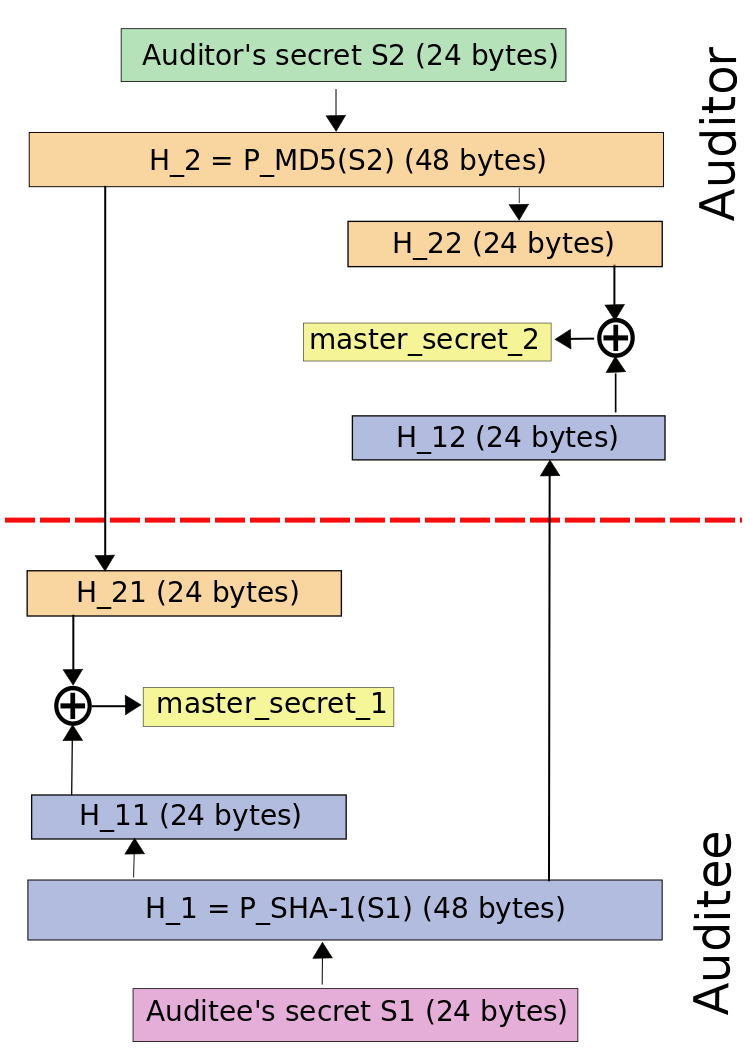
\includegraphics[scale=0.3]{PMS_to_MS.png}
\caption{\emph{Illustration of steps 1-7; the process by which secrets S1 and S2 are converted into two disjoint halves of the master secret for the TLS session. Data below the red dotted line is known to the auditee, that above the line is known to the auditor.}}
\end{figure}

\begin{enumerate}
\setcounter{enumi}{\theenumTemp}
\item The auditee now calculates 140 bytes: $X = \textrm{P\_MD5}(M_1)$
\item The auditor now calculates 140 bytes: $Y = \textrm{P\_SHA-1}(M_2)$
\item The auditor now gives to the auditee approximately 120 bytes of $Y$ (the exact number of bytes required is a function of the cipher suite used), allowing the auditee to immediately compute the IVs, the encryption keys and the client mac key (or `client write mac secret'). The auditee is now able to send the request to the server.
\item The server response is received but \underline{not} decrypted (or even passed into a browser). The network traffic is logged and a hash of this traffic is computed and sent to the auditor as a commitment.
\item Only when the auditor receives this commitment does he send the remaining 20 bytes of $Y$ to the auditee, allowing the calculation of the server mac key. The auditee can then safely execute a normal TLS decryption step (with authentication).
\end{enumerate}

These steps are illustrated in Fig 2.

\pagebreak

\begin{figure}[h]
\centering
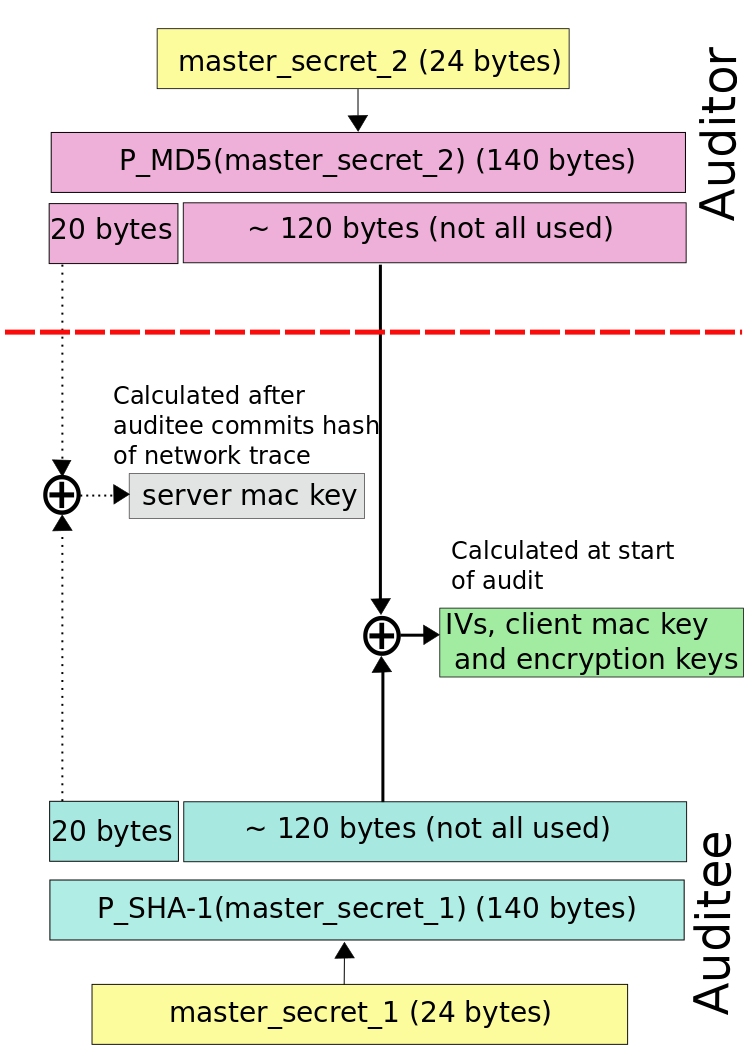
\includegraphics[scale=0.3]{MS_to_keys.png}
\caption{\emph{Steps 8-12. Conversion of 2 master secret halves into the expanded key block as described in Section 6.3 of the RFC. The server mac key (`server write mac secret' in the RFC) is withheld from the auditee until the server response is retrieved over the wire (but not known to the auditor). The red dotted line has the same meaning as in Fig 1.}}
\end{figure}

\noindent In summary, the purpose of this rather complex sequence of steps is: the auditor withholds some of the secret data from the auditee (acting as client), so that the auditee cannot fabricate traffic from the server (since at the time of making his request, he does not have the server mac write secret). Once the auditee has a made a commitment to the encrypted content of the server's response to his request, the auditor can provide the auditee with the required secret data in order to construct the server mac write secret. Then, the auditee can safely complete the decryption and authentication steps of the TLS protocol, since at that point he has the full master secret. In this way, the auditee maintains the full TLS security model, although he was prevented from creating a fake version of the post-handshake traffic from the server - something he is always able to do if he has the full master secret in advance.

\vskip 0.2 in 
\noindent While this process does allow the auditor to withhold part of the final key block from the auditee until he has already received a server response, it leaves a huge problem unsolved: how can the encrypted premaster secret be sent to the server, if neither auditor nor auditee knows the full premaster secret?
\vskip 0.1 in 
\noindent Section 2.2 describes the solution to this problem.


\subsection{Constructing the encryption of the premaster secret}
\noindent In order to allow each party on the client side ('auditee' and 'auditor' as above) to possess a different part of the secrets used in TLS, we make use of the homomorphic property of RSA encryption:
\begin{center}
\[\left(\textrm{RSA}(x_1) \times \textrm{RSA}(x_2)\right) \textrm{mod}\ n = \textrm{RSA}(x_1 \times x_2)\]
\end{center}
\noindent with $n=pq$ being the RSA modulus, a 2048 bit number.
\vskip 0.1 in 
\noindent The RSA Encryption RFC 2313 \cite{RSA_spec} specifies that a random padding string should be prepended to the message to be encrypted (RSA encryption is not secure without padding). In particular, the message to be encrypted here is referred to as the \textit{premaster secret}, a string of 46 bytes of random data with 2 bytes of version number prepended.
\vskip 0.1 in 
\noindent The exact data to be passed to the RSA encryption algorithm, in the step of encrypting the premaster secret, therefore looks like this:

\begin{equation}\label{blockformat}
 00 || 02 || \ldots \textrm{205 bytes of padding} \ldots || 00 || S_1 || S_2  
\end{equation}
where the terms $S_1$ and $S_2$ are the 24 byte strings referred to in point 1 of the algorithm described in Section 2.1. Note that the first two bytes of $S_1$ are required to be 03 01, since this is a fixed version number.
\vskip 0.1 in 
\noindent Two points are worthy of note about this structure:
\begin{itemize}
\item The length of padding is fixed at 205 bytes because the data to be encrypted is fixed at 48 bytes.
\item Since this is a public key operation, the padding is not allowed to contain any zero bytes (see RFC 2313 Section 8.1).
\end{itemize}

\noindent At this point it should be clear that we are trying to construct two or more multiplicative factors so that, multiplying them together produces the exact structure shown in (1), thereby allowing the auditor to provide the auditee with one or more such factor in \textit{encrypted} form. The auditee will then be able to multiply this by the RSA encryption of his own similar factor or factors, and then send on the result of that multiplication, confident that he is actually sending the encrypted premaster secret as required by the TLS protocol.

\pagebreak

\noindent We begin by observing that, if we take $S_1$ and $S_2$ to be 12 byte strings rather than 24 byte as described above, then  the structure $(2^{8*36}S_1+1)(2^{8*12}S_2+1)$ has the desirable property of including 
\begin{equation*}
2^{8*36}S_1+2^{8*12}S_2+1=S_1||(12\ \textrm{zero bytes}) || S_2 ||( 11\ \textrm{zero bytes}) || 01
\end{equation*}
\noindent inside it (consider multiplication of $(12000000+1) \times (3400+1)$ in decimal). However this is clearly insufficient as the term $2^{8*48}S_1S_2$ is not large enough to act as the ($02||$ 205 byte padding) mentioned above. So we must introduce a padding term. There is  more than one way to do this; however, for reasons explained later, it is desirable that \emph{both} multiplicative factors contain a padding term. We therefore propose this structure:

\begin{equation}\label{expanded}
\begin{split}
(2^{k_P}P_1+2^{k_1}S_1+1)(2^{k_P}P_2+2^{k_2}S_2+1) &= 2^{2k_P} P_1 P_2 + 2^{k_P+k_1}P_2S_1 \\
					&+2^{k_P+k_2}P_1S_2 + 2^{k_P}(P_1+P_2) \\
					&+ 2^{k_1+k_2}S_1S_2 +2^{k_1}S_1+2^{k_2}S_2+1
\end{split}
\end{equation}

\noindent We proceed in two stages, first describing a naive version which gives the right overall structure without meeting all the requirements of the protocol, before refining it.

\subsubsection{Naive form}
\noindent Here $P_1$ and $P_2$ denote padding strings of length 80 bytes, $S_1$ and $S_2$ are as defined above, and the final three terms are exactly the 48 byte premaster secret as required by the protocol (note that they will contain 12 zero byte strings each, so that each of (auditor, auditee) protects their secrets with 12 bytes of entropy each. The values of $k_1$,$k_2$ and $k_P$ are $(8 \times 36)$,$(8 \times 12)$ and $(8 \times 48)$ respectively. It can be seen that in this way we can construct a 256 byte number for which the last (lowest-order) 48 bytes are unaffected by the padding, and more specifically, the last 12 bytes are known only to the auditor, while bytes 25-36 are known only to the auditee. 

\subsubsection{Detailed form}

\vskip 0.1 in
\noindent To completely meet the specifications of \eqref{blockformat}, we must do a bit more: the first two bytes of the entire string must be 0002 (which effectively means constructing a 255 byte string starting with 02), the last byte of the padding string must be 00 and the two bytes succeeding it must be 0301. This is achieved with some very slight modifications to the above structure. First, $S_1$ must start with the two bytes 0301, while $P_1$ should start with 01 and $P_2$ should start with 02. To provide additional security to the auditee, we give 13 bytes of entropy to the auditee and only 8 bytes to the auditor. Thus the entire factor for the auditee becomes of this format:
\begin{equation}\label{auditee_factor}
[ \ \textrm{79 bytes}\ P_1\ ||\ 00\ ||\ 03\ 01\ ||\ 13\ \textrm{random bytes}\ ||\ 32\ \textrm{bytes}\ 00\ ||\ 01 ] 
\end{equation}
while that for the auditor is of this format:
\begin{equation}\label{auditor_factor}
[ \ \textrm{79 bytes}\ P_2\ ||\ \textrm{25 bytes}\ 00\ ||\ 8\ \textrm{random bytes}\ ||\ 15\ \textrm{bytes}\ 00\ ||\ 01 ] 
\end{equation}
, the exact formats of $P_1$ and $P_2$ being discussed in the next section.

\vskip 0.1 in 
\noindent Obviously these are restrictions to the entropy of the secrets; instead of a single client sharing a 46 byte secret with the server, the client is now split into two parties holding 13 and 8 byte secrets respectively. This security implications are discussed in Section 3.  

\subsubsection{Randomized padding for armoring}
\noindent Remembering that we intend the auditor to pass the RSA encryption of his multiplicative factor $(2^{k_P}P_1+2^{k_1}S_1+1)$ to the auditee, and that further the auditee will pass the encryption of the product of both multiplicative factors to the server, thus exposing his own encrypted factor RSA$(2^{k_P}P_2+2^{k_2}S_2+1)$ to the auditor, it's clearly necessary that both factors are encrypted safely. For this reason the padding numbers $P_1$ and $P_2$ contain randomness. This can be achieved without altering any of the above structure, as long as the first byte in the 255 byte string constructed is $02$. We therefore make the first bytes of $P_1$ and $P_2$ be 0201 and 0101 respectively, ensuring that their product starts with 02. For reasons that will become clear in the next section, it is preferable not to make the entirety of the remainder of the padding strings random. The formats described below are therefore somewhat of a compromise, but contain substantial randomness:
\vskip 0.1 in 
\noindent Auditee - $P_1$:
\begin{equation}\label{auditee_padding}
[ \ 02\ ||\ \textrm{39 bytes}\ 01\ ||\ 39\ \textrm{random bytes} ] 
\end{equation}
\noindent Auditor - $P_2$:
\begin{equation}\label{auditor_padding}
[\ \textrm{40 bytes}\ 01\ ||\ 39\ \textrm{random bytes} ] 
\end{equation}

\vskip 0.1 in 
\noindent After applying all these modifications, \eqref{expanded} will yield a string of 255 bytes in line with the requirements of \eqref{blockformat}, and it will also be safe for the auditor to send his factor the auditee, and the auditee to the server, without the possibility of the other party decrypting it.

\subsubsection{Zero bytes in the padding}
\noindent The auditee, not being in possession of the secrets $P_2$ or $S_2$ by design, cannot know most of the terms listed on the RHS of \eqref{expanded}. It is therefore possible that the encrypted premaster secret be rejected if any of the bytes created in the PKCS padding region are zero, and the auditee cannot know this in advance. This is partly ameliorated by the use of the repeated byte 01 in the padding factors. A detailed analysis is beyond the scope of this paper, but the probability of one or more bytes in this padding region being zero, under the current scheme, is around 0.3.
\vskip 0.1 in
\noindent An invalid input to encryption will result in a connection reset. Note, however, that the possibility of connection failure can be removed \emph{entirely} by testing any negotiated premaster secret by attempting to complete a full handshake with an oracle, which in this case can be one or many highly reliable websites which allows TLS connections.

\section{Security Considerations}

\noindent By restarting TLS sessions at will, the client can isolate the single web page he or she would like to present to the auditor and keep the remaining pages (including login pages) private.
\vskip 0.1 in
\noindent This will restrict the amount of data, the sensitivity of the data and the length of time for which TLSnotary is operating. All of this greatly reduces the danger of any attack being effective.

\subsection{Preservation of the TLS security model}

\noindent The reader's attention is drawn to Steps 11-12 in Section 2.1; due to these steps, the auditee, acting as client in the TLS session, is not exposed to unauthenticated data, since at the time of decryption, he has the full master secret and session keys. Thus the level of security from the auditee's point of view is unchanged from a normal TLS session in as much as his trust is based on (a)the server certificate/public key and (b)the MAC used to authenticate.

\vskip 0.1 in
\noindent The auditor, on the other hand, has proof that the auditee did not fake the traffic since he has (a) the certificate/public key of the server and (b) the hash of the network trace, which includes MACs for the records generated by the server, \emph{before} the auditee had knowledge of the actual server mac secret/key (a 20 byte secret).

\vskip 0.1 in
\noindent However, the entropy of the secrets used to protect the connection is reduced compared to vanilla TLS 1.0. This is discussed in the next section.

\subsection{Possible Attacks}
\vskip 0.1 in
\noindent We consider three distinct threats: the auditor gaining control of the session, an external attacker attempting the same, and the auditee taking control of the auditor's secret in advance of the connection. We do \emph{not} consider the possibility of the auditor tampering with the data, since the auditor must be trusted not to tamper with evidence in order to carry out his function.

\subsubsection{Auditor gaining control of live session}

\noindent The auditee's secret $S_1$ is, from the auditor's perspective, protected by 13 bytes of entropy. When the encrypted premaster secret, which is a complicated version of RSA($S_1*S_2$) is sent to the web server, the auditor could in principle be sniffing the traffic and gain access to this data immediately. However, since the encrypted message is padded according to the standard \cite{RSA_spec}, and the auditor has no knowledge of most of that padding, there is no plausible way for him to gain access to the auditee's secret. The client is not expected to be using the session for timeframes greater than a few minutes. Considering this set of circumstances, we claim that an attack on the TLS session by the auditor is infeasible.

\vskip 0.1 in
\noindent An attempt to attack by decrypting after the session has been terminated makes no sense, as it would only decrypt exactly what the auditee has already provided to the auditor (remembering that the auditee uses a completely separate TLS session for the one page he has chosen to be audited).

\subsubsection{External attacker gaining control of live session}

\noindent From an external attacker's perspective, the traffic between auditee and server is defended against MITM and similar attacks in the same way as a normal TLS 1.0 session using an RSA ciphersuite, the only differences being: 
\begin{itemize}
\item the total number of bytes of entropy defending the master secret is now 21 instead of 46. This is more than necessary to defend a secret, but even if the attacker were able to decrypt traffic long after a session is complete, he can only gain access to information that the auditee has already decided is safe to give to an auditor (e.g. it does not contain credentials).
\item the attacker may (depending on the messaging architecture) be able to access the message RSA($S_2$) sent from auditor to auditee during session set up, as well as the auditee's message containing the encrypted premaster secret. However as has been previously discussed, these message are armoured with 39 bytes of random padding, and so are protected from decryption in largely the same was as a scheme like PKCS 1 v1.5. In particular, note that there is no possibility of padding oracle attacks in this usage scenario. 
\end{itemize}

\subsubsection{Auditee gaining control of auditor secret}
This attack is of a different, somewhat lower level of concern as it involves the auditee violating the rules of auditing/arbitration rather than the loss of security in a live TLS session. However, in order to achieve this the auditee would need to crack an 8 byte secret within a period of minutes, which is considered infeasible. However the auditor should be aware that his level of protection is only about 64 bits, and moreover the algorithm can easily be tweaked to distribute more entropy to the auditor and less to the auditee if that is deemed to be necessary.

\pagebreak

 \begin{thebibliography}{1}

  \bibitem{TLS_spec} "The TLS Protocol Version 1.0" http://www.ietf.org/rfc/rfc2246.txt
  \bibitem{RSA_spec} "PKCS \#1: RSA Encryption Version 1.5" \newline http://www.ietf.org/rfc/rfc2313.txt

  \end{thebibliography}
  
\end{document}